\chapter{Dynamic heterogeneity in single electron-transfer proteins}
\label{chapter:azurin}
\graphicspath{{./chapters/c4_azurin_sm/main/}}
%============================== MAIN =======================================
\begin{abstract}
	Conformational dynamics of proteins plays a crucial role in their biological activity. Single-molecule studies have revealed the spread of reaction rates of enzymes, which was not accessible in ensemble measurements.
	The energy landscape of an enzymatic reactions consists a large number of substates with a rugged energy landscape.
	However, the heterogeneous nature of dynamics obtained from the analysis of single-molecule traces and their generality is still hotly debated.
	Here we provide evidence of conformational heterogeneity in the complex formation of an electron-transfer protein, azurin, with redox-active partners.
	We characterize the electron-transfer dynamics of single azurin molecules from time traces, histograms of bright and dark times, and correlation functions of redox events. 
\end{abstract}
\newpage
%============================ Introduction =====================================
\section{Introduction}
Enzymes perform metabolic processes inside the cell with minimal energy requirements.
Conformational fluctuation of enzymes has got attention since the finding of non-exponential distribution of kinetic rates for an ensemble of myoglobin. \cite{frauenfelder1991the,ansari1985protein,stein1985a,henzler-wildman2007dynamic}
Conformational substates might hold the answer to the evolution of highly complex enzymes to perform efficient conversion of substrate to product.
Single-molecule spectroscopy has revealed the dynamic fluctuation of enzymes covering many orders of magnitude.\cite{lu1998single-molecule,yang2003protein,english2006ever-fluctuating}
However, the evidences of heterogeneity from the analysis of single-molecule time traces has been strongly debated.
Blank and coworkers have shown that the non-exponential distribution in the turn-overs of enzymes might be an artifact of the analysis of the time traces.\cite{terentyeva2012dynamic}
They showed that both threshold and change point analysis, to find transitions on a intensity time trace, lead to non-exponentiality in the distribution of turn-over times.


Dynamics of electron transfer in metalloproteins are also of high interest.\cite{marcus1985electron,dooley1981spectroscopic}
Efficient electron transfer in living cells is essential for energy metabolism and storage.
Metallo proteins are promising candidates for bio-electronic devices and efficient energy conversion as a biofuel.
Copper proteins along with iron proteins play a crucial role in the biological redox reactions. \cite{solomon2004electronic,solomon2001oxygen,peisach1974structural,canters1993engineering} 
Similar to enzyme-substrate complex formation, electron transfer occurs through the formation of a complex between a metallo(redox) protein and its redox partners.


Electron-transfer proteins are characterized by their electron-transfer rates and midpoint potentials.
Subtle changes in the structure of proteins may lead to variations in the electron-transfer rates.
Do redox proteins posses conformational substates in a particular oxidation state?
To look for heterogeneity, We will investigate electron-transfer rates of the redox protein azurin across many single molecules and of single azurins as a function of time.


Azurin is a copper protein  with molecular weight of \SI{\sim14}{\kilo\dalton}, which is believed to be taking part in redox homeostasis in cells.
A copper metal center is found in the so-called northern region of the protein matrix.
The surrounding ligands of the copper ion result in a $\pi-\pi*$ transition giving the protein a blue color (absorption in \SIrange{590}{620}{\nm}) in the Cu(II) state.
Cu(I)azurin is colorless due to the absence of the absorption band in the red.
The oxidation state of single azurin molecules can be determined by attaching a fluorophore whose emission overlaps with the absorption of Cu(II)azurin.\cite{kuznetsova2006a,kuznetsova2008the}
The fluorescence of the label strongly depends on the oxidation state of the copper.
In the Cu(II) state, the fluorescence is quenched while in the Cu(I) state the fluorescence is reserved.
The durations of high intensity bursts are denoted as bright times and the durations of low intensity bursts are denoted as dark times.


We study electron transfer in labeled single azurins while they react with electron mediators.
The redox potential of the solution is varied by applying an electric potential to a fixed concentration of electron mediators.
The distribution of electron-transfer rates across many single azurins was compared with the distribution of electron-transfer rate of a single azurin as a function of time.
The dynamics of single azurins was characterized by their intensity time traces, intensity correlations, histograms of bright and dark times, and the correlation of bright and dark times.

% \begin{itemize}
% 	\item Dynamic properties of enzymes have been focus of much research: Frauenfelder, Eaton, Onuchic, Kern. Single molecule: Xie HP Lu, H. Yang, van Oijen, Hofkens, Blank, Goldsmith
% 	\item Also the dynamic properties of ET proteins are of high interest: Marcus, Canters, Eaton
% 	\item Characteristic of ET-redox proteins are E0 and ET kinetics.
% 	\item Question: are these properties distributed in an ensemble and if so in what sense. Ergodicity, time and ensemble averages: Barkai
% 	\item We have investigated this by studying the E0 and the k's by SM techniques
% 	\item Do this by applying electric potential and looking at life times of reduced and oxidized state.
% 	\item Can do this by fluorescent labeling because the fluorescence is strongly dependent on the oxidation state through FRET.
% 	\item We will show that $...$
% \end{itemize}
%%%%%%%%%%%%%%---------- EXPERIMENTAL SECTION ----------%%%%%%%%%%%%%%%%%%%%
\section{Experimental section}

\paragraph*{Protein synthesis.}
Azurin (wild type) from \textit{Pseudomonas aeruginosa} was expressed in \textit{E. Coli} and purified as described before \citep{kamp1990purification}.
BL21 \textit{E.coli} cells were transformed with the PGK22 plasmid that carries the gene for azurin.
The cells were cultured in Luria Bertani (LB) medium.
Then the cells were harvested and resuspended in a \SI{20}{\percent} (w/v) sucrose solution in Tris pH 8 buffer containing \SI{1}{\mM} EDTA.
The solution was centrifuged (\SI{8000}{ rpm}, \SI{20}{\minute}) and the supernatant was collected.
Copper sulfate was added to the solution for insertion of Cu into the active site of azurin.
The unwanted proteins were precipitated by addition of concentrated acetic acid until pH 4. 
The turbid solution was centrifuged at \SI{8000}{ rpm} for \SI{20}{\minute}.
The supernatant was loaded on a CM Sepharose fast flow column and elution was performed in an Akta purifier (GE Healthcare) with a pH gradient from 4 to 6.9 in 
\SI{50}{\mM} ammonium acetate.
Fractions containing azurin (inferred from the absorbance at \SI{290}{\nm} and \SI{620}{\nm}) were collected and reduced with sodium dithionite.
At this stage the solution contained both zinc and copper azurin.
The azurins were purified in a DEAE sepharose column by a salt gradient of 0 to \SI{50}{\mM} NaCl in Tris pH8 buffer. 
Fractions containing copper azurin and zinc azurin were collected and concentrated separately.
The purity of the samples was checked by gel electrophoresis (PAGE, on polyacrylamide gel with sodium dodecyl sulphate, SDS) and by UV/Vis spectroscopy (Cary 50 spectrophotometer, Varian Inc., Agilent Technologies, USA).
The azurin was further appeared on SDS gel PAGE at $\sim$\SI{14}{ kDa}.
Both zinc and copper azurin showed a characteristic shoulder at ${\sim}$\SI{290}{\nm} while Cu azurin showed an additional 
broad absorption peak at \SI{620}{\nm} when oxidized, as can be seen in Figure-S\ref{SIfig: switching}. 
The ratio $OD_{\SI{628}{\nm}}/OD_{\SI{280}{\nm}}$ for Cu azurin was 0.56, which indicated a purity of more than \SI{95}{\percent}. 
The concentrated protein was stored at \SI{-80}{\celsius} until further use.


\paragraph*{Fluorescent labeling.}
The labeling protocol was based on previous work \cite{nicolardi2012topdown}.
ATTO655 NHS-ester was bought from ATTO-TEC GmbH and used without further purification.
The azurin solution was equilibrated with HEPES pH 8.3 for a higher efficiency of the amine-NHS-ester reaction.
ATTO655 was chosen to label the protein because of its photostability and inertness (unreactive) to the redox chemicals used in the study.
A mixture of \SI{200}{\uM} azurin and ATTO 655 NHS-ester (1:1) was incubated for \SI{45}{\minute}.
The NHS-ester group reacts with one of the amine groups on the protein.
The unreacted dyes were removed with a HiTrap desalting column.
The labeled protein was concentrated in Tris pH 8.5 buffer by centrifuging in a \SI{3}{ kDa} Amicon ultra-filter.
The labeled protein was further purified by ion exchange chromatography in a \SI{1}{\mL} MonoQ column (GE Health).
The different peaks obtained (see Figure S\ref{SIfig: peak_sep}) correspond to different numbers and positions of the dye on the azurin surface. 
Peak III corresponds to proteins labeled at Lysine122 position \cite{nicolardi2012topdown}.
For this position of the dye, the protein construct shows a high fluorescence switching ratio \SI{90}{\percent} between oxidized and reduced conditions as can be seen in Figure S\ref{SIfig: peak_sep}. This fraction was chosen for our single-molecule experiment as the two states can be distinguished easily.
The same protocol was used for Zn-azurin labeling and similar peak separations were observed.
The fluorescently labeled proteins were then reacted with biotin-PEG-NHS (MW 3400) in phosphate-buffered saline (PBS) pH 7.4 buffer with a ratio 1:5 (azurin : biotin-peg-NHS) to make sure each protein has at least one biotin.
The free biotin was then removed by centrifuging in a \SI{3}{ kDa} Amicon ultra-filter.
The biotin on the protein will be used for immobilization on the glass surface.


\paragraph*{Functionalization of coverslips.}
The functionalization of the glass surface was achieved according to previous work with slight modifications.\cite{gupta2012involvement}
Glass coverslips (Menzel-Glaser, $\SI{22}{\mm} \times \SI{40}{\mm}$, no. 1 thickness) were used for immobilization.
The coverslips were sonicated in water (\SI{15}{\minute}) and acetone (\SI{15}{\minute}).
Then they were rinsed in Milli-Q water several times and incubated in a \ce{H2O}/\ce{NH4OH}/\ce(H2O2)(5:1:1) bath at \SI{70}{\celsius} for removing organic impurities from the surface.
The coverslips were rinsed several times with water and ethanol and finally stored in ethanol.
Before functionalization, the slides were flamed and treated for \SI{30}{\minute} with a \SI{1}{\percent} solution of [3-(2-aminoethyl)aminopropyl] trimethoxysilane in methanol containing \SI{5}{\percent} glacial acetic acid. This results in the binding of the silane to active hydroxyl groups.
At this stage the silane is not yet covalently bound, but this is achieved by baking the cover slips in an oven at \SI{65}{\celsius} for \SI{3}{\hour}.
After this treatment, the coverslips were sonicated for \SI{10}{\minute} and washed with methanol.
Dried with clean nitrogen, they were left in a desiccator overnight. 
The next day they were treated with a mixture of \SI{5}{\mg\per\mL} methoxy-PEG-N-hydroxysuccinimide (MW~2000, Laysan Bio) and \SI{0.05}{\mg\per\mL} biotin-PEG-N-hydroxysuccinimide (MW 3400, Laysan Bio) in \SI{50}{\mM} phosphate buffered saline (PBS), pH 7.4.
This creates a surface containing biotin and methoxy end groups.
The PEG surface prevents nonspecific adsorption of the protein.
The slides were dried with a gentle flow of nitrogen and stored in a desiccator until further use.


\paragraph*{Protein immobilization.}
The biotin-functionalized glass slide was incubated with \SI{20}{\mM} PBS pH 7.4 buffer for \SI{5}{\minute}.
\SI{100}{\nM} of NeutrAvidin (Thermo Scientific) was incubated for another \SI{15}{\minute} and then washed to remove unbound NeutrAvidin. 
Then \SI{100}{\pM} of the labeled protein was incubated for \SI{1}{\minute} to get isolated proteins (20 per \SI{100}{\um} area) to bind to the functionalized glass surface.
The unbound proteins were then removed by washing with fresh PBS pH 7.4 buffer.


\paragraph*{Electrochemical-potential control.}
Once the unbound proteins were removed, a new mixture containing \SI{0.1}{\mM} sodium ascorbate (\ce{C6H7O6-Na+}) and \SI{0.2}{\mM} potassium ferricyanide (\ce{[Fe(CN)6^3-]}) was added to PBS pH 7.4 to get a total volume of \SI{4}{\mL}.
The redox potential of the solution was controlled by a potentiostat (Model 800B Series Electrochemical Detector, CH Instruments) with the same electrochemical setup as previously described\cite{zhang2017gold} with little modification.
A square platinum grid (grid side \SI{2.5}{\cm}) was used as working electrode and pressed onto the sample slide with the help of a small glass slide.
The voids of the grid are closed by the glass slides, forming small confined volumes where the sample slide and glass slide are the `floor' and `roof' and the platinum grid forms the `walls'.
These confined volumes are in the order of nanoliters, which makes switching of the electrochemical potential of the solution possible in a matter of minutes.
The change in the solution potential changes the concentration of reductant and oxidant that can be calculated with the help of the Nernst equation.


\paragraph*{Confocal Microscope.}
Single-molecule measurements were carried out in a home-built confocal microscope.
The setup was equipped with a \SI{635}{\nm} pulsed diode laser (Power Technology, Little Rock, AR, USA) controlled by a PDL 828 "Sepia II" (PicoQuant) at \SI{40}{\MHz} repetition rate.
The laser beam was passed through a narrow-band cleanup filter (Semrock LD01-640/8-25) and coupled to a single-mode optical fiber to obtain a Gaussian beam profile.
The output beam was collimated and reflected by a polychroic mirror (z488/633rpc) onto the back aperture of an oil immersion objective (NA=1.4, Olympus UPLSApo 100x).
The sample holder with the glass slide and electrodes was mounted on a scanning stage (Physik Instrumente P-517.3CD) controlled by a nanopositioning system (Physik Instrumente E-710.3CD). 
The epifluorescence light was collected back through the same objective and focussed on a \SI{50}{\um} pinhole for spatial filtering, then the light passed through an emission filter (z488/635m "dual"-band emission filter, Chroma). 
The fluorescence beam was re-collimated and focussed on a single-photon avalanche photodiode (SPCM AQRH-15, Perkin Elmer Inc., USA).
The signal from the photodiode was recorded by a PicoHarp 300 (PicoQuant GmBH, Berlin, Germany) in time-tagged-time-resolved mode.

%Scheme
\begin{figure}
	\centering
	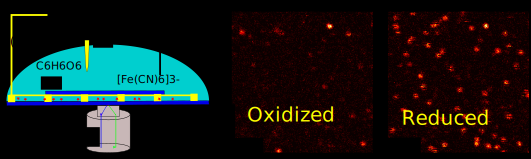
\includegraphics[width=\textwidth]{Scheme_1_setup}
	\caption{Scheme of the confocal and electrochemical setup.
	\textbf{(1)} Objective through which light is irradiated on and collected from the sample.
	\textbf{(2)} Functionalized sample slide with another small glass slide on top the platinum grid.
	\textbf{(3)} Electron mediator solution containing \SI{200}{\uM} ferricyanide, \SI{100}{\uM} ascorbate in PBS (pH 7.4) buffer with a total volume of 4 mL.
	\textbf{(4)} Working electrode (platinum wire) that is in contact with the platinum grid (yellow blocks) with a height of \SI{50}{\um}.
	\textbf{(5)} Saturated calomel reference electrode (SCE).
	\textbf{(6)} The platinum wire (not touching the grid) as counter electrode.
	\textbf{(7)} Potentiostat (Model 800B Series Electrochemical Detector, CH Instruments) to which the electrodes are connected.
	Zoom-in picture shows the functionalization method and the working electrode around it. 
	\textbf{(8, 9)} Confocal scanning images of the surface of the substrate at \SI{100}{\mV} (oxidizing) potential and \SI{0}{\mV} (reducing) potential.
	The spots on the left side (8) are impurities/bleached proteins.
	}
  	\label{sch:setup}
\end{figure}
\paragraph*{Data recording.}
A \SI[product-units=repeat]{20x20}{\um} area of the sample surface functionalized with sparsely distributed ATTO655-labeled azurin was scanned with \SI{50}{\nm} per pixel and with a dwell time of \SI{1}{\ms} per pixel.
A typical fluorescence intensity image can be seen in Scheme \ref{sch:setup}.
A constant potential of \SI{200}{\mV} vs SCE (oxidizing) was applied by the potentiostat and an image of \SI[product-units=repeat]{10x10}{\um} area was taken after \SI{2}{\minute}.
Typically within one minute, the solution potential of the mixture of \SI{0.1}{\mM} ascorbate and \SI{0.2}{\mM} ferricyanide reaches the applied potential.
Another image of this same area was recorded at \SI{0}{\mV} (reducing).
The two images were compared to identify the active molecules, which switch to a bright and dark at the two potentials (Scheme-\ref{sch:setup} (8 \& 9)).
The coordinates of the switching molecules were registered and an automatic recording was started.
For each molecule, time traces were recorded for \SI{30}{\s} at different potentials between \SI{-100}{\mV} and \SI{100}{\mV}.
To observe the dynamics of a single molecule over longer times, time traces were recorded until the dye was  bleached or the protein was denaturated.
Zn-azurin-ATTO655 was used as a control since it does not show switching at the above potentials.
Time traces at the same potentials for the same durations were recorded as for the Cu-azurin.


\paragraph*{Data analysis.}
The measurements resulted in more than a 1000 time traces.
Each time trace contains the absolute arrival times of photons as well as the arrival time with respect to the excitation laser pulse.
This enabled us to extract maximum information from the traces.
To minimize accidental variation and improve efficiency, codes were written (in Python and Matlab) to standardize the analysis of the time traces.
% The codes and data can be found in the given link (will be provided during submission).
Each trace was analyzed in three ways (i) Intensity change points in the time traces were obtained using the Change-Point algorithm\cite{watkins2005detection} provided by prof. Haw Yang 
(Princeton University, USA).
This method is bin-free and does not require any prior knowledge of the underlying kinetics.
It determines the location of intensity changes based on the photon arrival times and the algorithm is recursively applied over the whole time trace to find all the changes.
A Bayesian information criterion is used to find the number of states.
In the present case two states were identified from long time traces of many molecules (2500 change points each) with a reported accuracy of more than \SI{90}{\percent}.
This is in agreement with our expectation of two states, namely a Cu(II)-quenched (low intensity) and a non-quenched Cu(I) state (bright).
Consequently the number of states for the other time traces has been set to two to minimize the computation time.
An example of a trace with change points and its overlap with the real time trace can be seen in Figure-\ref{fig:timetrace}.
(ii) Autocorrelation functions of the time traces were calculated using the SymPhoTime(PicoQuant) software.
(iii) Further analysis of Change-Point outputs and the autocorrelation outputs were performed in Python.
% The details of the code including all the fitting functions can be found in the online repositories (will be provided during submission).


%%%%%%---------------------RESULTS and DISCUSSION-----------------------%%%%%%%%%
\section{Results and discussion\label{sec:results}}
\paragraph*{Time traces at different potentials.}
Active Cu-azurin molecules were identified from their fluorescence intensity images under oxidizing (\SI{200}{\mV}) and reducing conditions (\SI{0}{\mV}).
In reducing conditions, the image contains many bright spots corresponding to Cu(I)-azurin-ATTO655 and more than \SI{90}{\percent} of these molecules are turned off in oxidizing conditions 
(Scheme-\ref{sch:setup}(8)).
The azurins on each sample slide showed active switching during the course of the experiment (up to two days) without any noticeable degradation.
A set of active azurins were marked for recording, and time traces at different potentials (between \SI{-100}{\mV} and \SI{100}{\mV}) were measured on the \texttt{same molecule} 
for \SI{30}{\s}.
Many of the labeled proteins bleached during the recording at the first few potentials, but more than \SI{50}{\percent} of the labeled azurins survived at least five measurements (\SI{150}{\s}  total) at different potentials.
Longer measurements were possible thanks to the scavenging of oxygen in the solution.
Indeed, before recording the time trace, the solution was exposed to a negative potential for at least \SI{1}{\hour}.
Ascorbate is known to  scavenge oxygen\cite{dave1997effectiveness} and get oxidized.
The oxidized ascorbate is then reduced by the electrode and is again available to scavenge other oxygen molecules.
% In addition to the absence of oxygen, the  oxidizing-and-reducing-system (ROXS) mechanism was also at play.\cite{cordes2009on}
The reduction and oxidation of Cu-azurin made the dye switch from bright to dark fluorescent states. Under oxidizing conditions, the dye spent less time in the bright state, and the bleaching rate was reduced.
We could measure some fluorescence time traces for more than \SI{1000}{\s}.\\
%---time trace
\begin{figure}
	\centering
	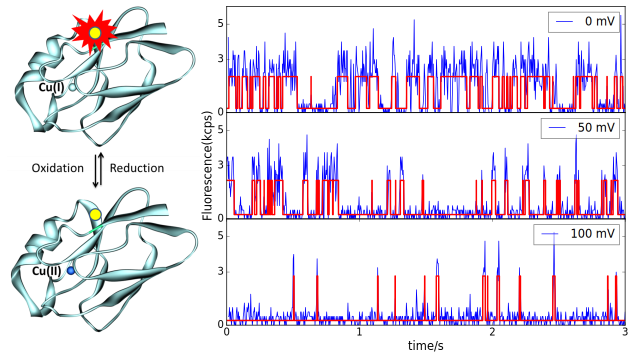
\includegraphics[width=\textwidth]{Figure_1_timetrace_CuAzu}
	\caption{Time traces of the same Cu-azurin-ATTO655 at different potentials (0, 50 and \SI{100}{\mV} with respect to SCE).
	The structure of the protein with properly positioned dye can be seen in the schematic picture in the left.
	In the Cu(II) state (shown as blue dot in the protein structure), the dye is non fluorescent because of FRET and in the Cu(I) state (shown as as a gray dot), the dye is fluorescent. Notice the amount of time the protein spends in the bright and the dark state at different potentials.
	At lower potentials (e.g \SI{0}{\mV}) the protein is bright most of the time because of the higher concentration of reductant.}
	\label{fig:timetrace}
\end{figure}


Figure \ref{fig:timetrace} shows time traces of a single Cu-azurin-ATTO655 molecule at three different potentials. 
The intensity changes from bright to dark and vice versa over time.
In the dark state, the dye fluorescence is quenched by energy transfer to the absorbing Cu(II) center\cite{kuznetsova2006a}.
The high FRET efficiency is due to the small distance of the dye to the absorption center.
This clear distinction between the dark and bright states is important to clearly distinguish redox states, even for low laser power and low signals.
At higher potential (\SI{100}{\mV}), the protein spends most of its time in its dark state and as the potential is lowered, the molecule spends more and more time in its bright state.
Bulk (ensemble) measurements of the fluorescence intensity under completely oxidizing and completely reducing conditions shows \SI{90}{\percent} switching ratio (Figure S\ref{SIfig: switching}) for the lysine-122 labeled Cu-azurin-ATTO655.\cite{nicolardi2012topdown}
In the single-molecule traces in Figure \ref{fig:timetrace}, no clear fluorescence signal from the quenched state could be detected.
However, residual fluorescence from the quenched state can be observed at higher laser power (\SI{0.7}{\uW}) as can be seen in (Figure S\ref{SIfig: lifetime}).
This proves that the observed intensity changes are not due to blinking of the dye, but due to incomplete (\SI{90}{\percent}) quenching by the copper center. 
We also note that the Cu(II)-state has a much shorter lifetime (\SI{0.3}{\ns}) than the Cu(I)-state (\SI{1.9}{\ns}), but still significantly longer than the instrument response function (\SI{0.2}{\ns}). 
Both measurements of intensity and lifetime indicate that the dim state is quenched by energy transfer to Cu(II), in agreement with bulk fluorescence measurements on Cu-azurin.


Figure \ref{fig:timetrace} also shows that bright times shorten at larger electrochemical potential.
This agrees with the higher oxidant concentration in the solution. 
A control study with Zn-azurin-ATTO655 (Figure S\ref{SIfig:tracecomparision} and Figure S\ref{SIfig:fcscomparision}) shows that the dye itself blinks below \SI{40}{\mV}.
Zn-azurin is inert to redox changes and thus the blinking can only originate from the interaction of the dye with the reductant through photo-excited electron transfer.
To exclude redox reactions of the dye itself, we only considered potentials above \SI{40}{\mV} for the Cu-azurin-ATTO655 study.


%Midpoint histogram
\paragraph*{Midpoint potential of single azurins.}
Figure \ref{fig:midpoint}a shows the ratio between the average dark time ($\me{t}_{d}$) and average bright time ($\me{t}_{b}$) plotted against the applied potential.
The relationship of this ratio with the potential is given by the Nernst equation: 
\begin{equation}
	E = E_0 - \frac{k_BT}{n e}\ln\left(\frac{\me{t}_{b}}{\me{t}_{d}}\right)\,
	\label{eq:nernst}
\end{equation}
where $E$ is the applied potential, $E_0$ the midpoint potential, $k_B$ the Boltzmann constant, $T$ the absolute temperature, $n$ the number of electrons involved in the reaction and $e$ the electron charge.
The value of $n$ was found to be $1$ from the data analysis when the slope in the Nernst equation was kept as a free parameter (see Figure-S\ref{SIfig:potential_slope}).
Each color represents a single azurin molecule and the solid line connecting the points is the fit with the Nernst equation.
Labeled proteins surviving at least three potentials above \SI{40}{\mV} were used for the fit.
The potential at which the bright-dark  ratio equals $1$ is the midpoint potential.
The distribution of midpoint potentials (Figure \ref{fig:midpoint}b) from \SI{132}{ molecules} can be fitted by a Gaussian with a center value of $\left<E_0^{SM}\right>=4.5 \pm 1.2~mV$ and a full width half maximum (FWHM) of $\sigma^{SM}=36 \pm 3~mV$. 
The midpoint potentials are similar to previously reported values of $6\pm0.6~mV$ with $FWHM=\SI{150}{\mV}$ where each $E_0$ was calculated from a cluster of about \SI{1000}{ molecules}.\cite{davis2006monitoring}
Another work reported $E_0 = \SI{16}{\mV}$ with low surface coverage (100's of azurins) with a FWHM of \SI{70}{\mV}.\cite{salverda2010fluorescent} 
Recently, for single azurin molecules, a midpoint potential of $E_0=12\pm3$ was reported with a FWHM of \SI{92}{\mV}.\cite{akkilic2014chemically-induced}\\
\begin{figure}
	\centering
	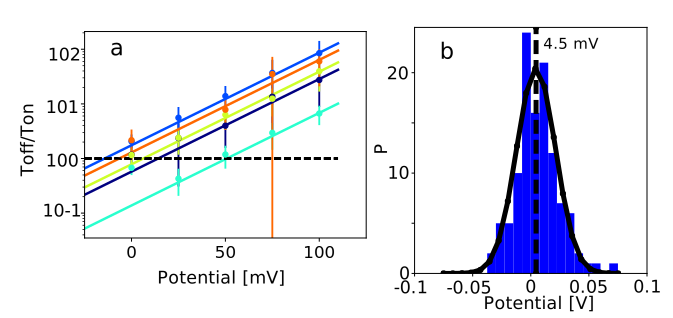
\includegraphics[width=\textwidth]{Figure_2_midpoint}
	\caption{Ratio between bright and dark times as a function of applied potential for the same single azurin.
	Different colors represent different single molecules.
	The line connecting the data points is the Nernst fit with $n=1$ for all the data points above \SI{40}{\mV}.
	The plot at the right is the histogram of midpoint potentials for \SI{132}{ molecules} with a Gaussian fit with a center value of \SI{4.5}{\mV} with respect to the calomel electrode.}
	\label{fig:midpoint}
\end{figure}

The distribution of midpoint potentials we find for single azurin is narrower (FWHM \SI{36}{\mV}) than in earlier measurements. We attribute this narrow distribution to a weaker interaction with the surface. Indeed, in our experiment, the proteins were functionalized through a PEG tether with a length of ${\sim}\SI{20}{\nm}$ itself attached to the surface by a NeutrAvidin. The total tether length is much longer than in earlier experiments, where the azurin was either non-specifically attached to the surface, or attached through a very short linker (\SI{<1}{\nm}).
In addition, the PEG passivation of the glass surface minimizes the interaction of the protein with the surface. Indeed, no protein was found to bind to the surface if the neutravidin was taken out, showing the absence of non-specific interactions.

%====================Many single-molecule on-off histogram and their rates=================
\paragraph*{Redox reaction rates from histograms of bright and dark times.}
\begin{figure}
	\centering
	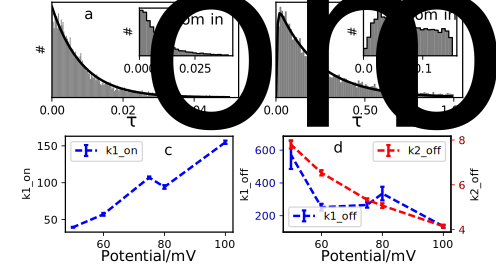
\includegraphics[width=\textwidth]{many_sm_hist}
	\caption{\textbf{Electron transfer rates (many molecules)} The histogram of bright times (a) and dark times (b) obtained from 132 single-Cu-azurin-ATTO655 molecules at \SI{100}{\mV}. The inset shows a magnified part for short times.
	The bad fit of the histogram of bright times with a single-exponential function shows its  non-exponentiality.
	Similarly the histogram of dark times shows non-exponential decay but with a buildup (rise time) at the begining.
	A possible interpretation is that reduction of Cu-azurin occurs through an intermediate step while for oxidation no intermediate state is observable.
	(c) Oxidation rate constant as a function of potential. 
	(d) Reduction rate constant as a function of potential: blue points correspond to the faster rate constant (rise, $k_2$) while the red points represent the slow rate constant ($k_3$).}
	\label{fig:many_sm_hist}
\end{figure}
The number of bright-dark switching events for a single azurin molecule was limited by fluorescence bleaching and led to noisy distributions.
For this reason we first analyzed the overall distribution of bright- and dark-times of all the single molecules obtained at a certain potential, which basically can be considered as an ensemble measurement.
Figure \ref{fig:many_sm_hist}(a) shows the histogram of bright-times at \SI{100}{\mV} and the solid line is the fit of a single exponential with a time constant ($k_{1}$) of \SI{155}{\per\s}.
The on-time represents the time the protein spends in the reduced state before getting oxidized according to the following reaction scheme:
\begin{align}
	\ch{!(bright)(Cu(I)Az) + ox <=>[ $k_1$ ][ $k_{-1}$ ] !(dark)(Cu(II)Az) + red }
	\label{eq:oxidation}
\end{align}
In contrast, the distribution of bright-times shows a maximum with a buildup and decay (Figure \ref{fig:many_sm_hist}(a)).
The inset with binning time \SI{5}{\ms} clearly shows that the probability of finding very short bright-times is relatively small.
This distribution can be explained with the Michaelis-Menten mechanism:
\begin{align}
	\ch{!(dark)(Cu(II)Az) + red <=>[ $k_2$ ][ $k_{-2}$ ] !(dark)(Cu(II)Az.red) -> [ k3 ] !(bright)(Cu(I)Az) + ox}
	\label{eq:reduction}
\end{align}
where $k_2$ is the pseudo-first order rate constant, which depends on the concentration of reductant and $k_3$ is the zero order rate constant, which should be independent of the concentration of the substrate.
When assuming $k_{-2}=0$, the probability distribution of bright times is given by\cite{lu1998single-molecule}
\begin{equation}
	P(t_{d}) = \frac{k_2k_3}{k_3-k_2} [exp(-k_2t_{d})-exp(-k_3t_{d})]
	\label{eq:2exp_risetime}
\end{equation}
At \SI{100}{\mV}, $k_2$ for the reduction is \SI{4.1}{\per\s} while $k_3$ is \SI{135}{\per\s}.
The data doesn't match with a single component distribution, which is not surprising as the distribution is built from many single azurins and each azurin has its own decay.
Similar to the distribution in midpoint potential, the non-exponential decay is a reflection of the statistical heterogeneity among the azurins.

The oxidation and reduction rates were determined at different applied potentials.
As expected, the rate constant for the intermediate complex formation ($k_2$) is dependent on the substrate concentration and thereby the potential while the rate constant for electron transfer in the intermediate is independent of the potential (Figure \ref{fig:many_sm_hist}(c)).
The rate of complex formation can be modeled as:
\begin{equation}
	k_3 =k_3^0\times[R] \text{ and } k_1 =k_1^0\times[Ox]
	\label{eq:rate_complex}
\end{equation}
\begin{equation}
	[R] = \frac{R_0exp(\frac{E_0^R-E}{0.059})}{1+exp(\frac{E_0^R-E}{0.059})}
	\text{ and } [Ox] = \frac{O_0}{1+exp(\frac{E_0^O-E}{0.059})}
	\label{eq:conc_potential}
\end{equation}
$[R]$ is the concentration of reductant (equivalent to ``substrate'' in enzymology), $R_0$ is the starting concentration of reductant which is equal to the concentration of ascorbate in this case, $E_0^R$ is the standard redox potential of ascorbate that is \SI{30}{\mV} and $E$ is the applied potential. The value $0.059$ stands for $\frac{RT}{nF}$ similar to the slope in the Nernst equation(Eq. \ref{eq:nernst}) with $n=1$.
Similarly $[Ox]$ represents the concentration of the oxidant (ferricyanide) at different applied potentials.
The maximum rate constant of reduction ($k_3^0$) was obtained to be $3.3\times10^5~M^{-1}s^{-1}$ while the maximum rate constant of oxidation was $1.3\times10^8~M^{-1}s^{-1}$.


However, Terentyeva et al. have shown that the presence of a rise time in the bright-time distribution can be an artifact in the changepoint analysis.
Our initial simulations and change point analysis indicates the underestimation of short dark times but not the extent that can give a rise time.
Our interpretation of the build-up in the histograms is thus under further investigation.

%==================Dynamics: Single-azurin over time===================
\paragraph*{Dynamical heterogeneity.}
After studying ${\sim}150$ single azurins together in an ensemble fashion, we investigated single azurins for as long as their fluorescence survived.
Figure \ref{fig:long_azurin_trace} shows the statistics of a single azurin at \SI{100}{\mV} that survived for \SI{\sim350}{\s}.
Two different parts of the original time trace (\ref{fig:long_azurin_trace}C), indicated by colored blocks, are magnified and shown in Figure \ref{fig:long_azurin_trace}A and B.
The two zoomed-in traces have very different bright-dark characteristics.
The one on the left has short bright-times and long dark-times while the one on the right has long bright-times and short dark-times.
The full time trace was divided into small parts and the average was calculated over every $10$ consecutive bright and dark times (Figure \ref{fig:long_azurin_trace}E,G).
We averaged over 10 points to reduce noise (see SI Fig S\ref{SIfig: N_avgpoints_vs_fwhmwidth}) and highlight the difference between the two parts of the trace.
Unlike random (Gaussian) noise, spikes and correlated high-low events are observed on the trace, which is also reflected in the density of points per unit time.
Longer bright and dark times result in a lower density of points.
The histograms of bright and dark times are shown on the left side of the trace without any averaging and the fit is shown with a single exponential function.
The distribution of dark times is clearly non-exponential as can be seen from the big deviation from the exponential fit.
Surprisingly, the histogram of bright times fits well with an exponential function even though the trace of bright times shows clear variation. 
The trace of midpoint potential (Figure \ref{fig:long_azurin_trace}I) is calculated through the Nernst equation for each point on the trace and with the applied potential.
The midpoint potential in the trace also fluctuates in a non-Gaussian way which can also be seen in the shape of its distribution (Figure \ref{fig:long_azurin_trace}H) with an average value of \SI{42.2}{\mV}.
%long_azurin_trace
\begin{figure}
	\centering
	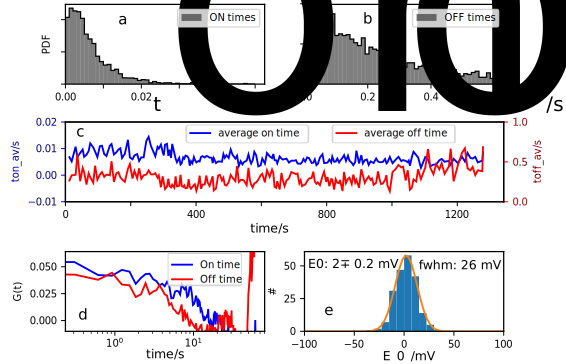
\includegraphics[width=\textwidth]{long_azurin_trace}
	\caption{\textbf{Dynamic heterogeneity.}
	A long time trace (C) of Cu-azurin-ATTO655 at \SI{100}{\mV} with zoom-in (A, B) at different points of its time course.
	Variation of bright times (E) and dark times(G) of the same azurin with their histogram on the left.
	The times were averaged over every ten consecutive ones to get rid of noise and for easy visualization.
	The trace of midpoint potential(I) calculated from the bright- and dark-times and the the histogram(H) of midpoint potential is shown on its left with an average value of \SI{42}{\mV}.
	}
	\label{fig:long_azurin_trace}
\end{figure}


The heterogeneity in the bright and dark times is related to the heterogeneity in the rate of electron transfer, particularly the longer times, which presumably is the rate of intermediate-complex formation.
The first explanation of heterogeneity we should consider is the effect of the surface.
Previous studies have shown that the azurin can stick to hydrophobic surfaces through the different hydrophobic patches on the protein surface.\cite{patil2010visualizing,salverda2010fluorescent,akkilic2014chemically-induced}
However, special care was taken to keep the protein as far as possible from the surface through a long (\SI{\sim20}{\nm}) PEG-linker, and to passivate the surface with short PEG ligands.
Indeed, no azurin was found attached to the surface of the substrate when the labeled azurin was flown onto the surface without NeutrAvidin or Biotin (everything else in the functionalization method kept the same) indicating the absence of non-specific interactions between the protein and the surface.
The narrow distribution (narrower than any previous measurements) of midpoint potentials among the 132 single azurins (Figure \ref{fig:midpoint}) also confirms the absence of interaction with the surface.
From these observations, we conclude that the surface contribution to the heterogeneity can be ignored.
We can also rule out concentration fluctuations of reductant and oxidant, as the solution potential is precisely controlled by the potentiostat.


The heterogeneity in the rates can now only be attributed to conformational changes of the protein.
Midpoint potential changes (\SI{<4}{\kJ\per\mole}) are much smaller than the changes in the free energy (\SI{-23}{\kJ\per\mole}, $\Delta{G}=-nEF$) related to the change in the oxidation state of azurin.
Such small changes can be attributed to subtle changes in the structure of the protein, each of these sub-structures are called conformational sub-states.

%XXXX Think about the argument XXXX


The protein remains in certain conformational sub-states for a duration of time, which can be observed in the time trace.
A short bright-time followed by a short bright-time represents one state while a long bright-time followed by a long bright-time represents another sub-state.
The residence time in each of these conformational sub-states can be characterized by autocorrelating the time trace of bright and dark times (Figure \ref{fig:Dynamic_corr} A).
The characteristic correlation times are in the order of $1-10$ of seconds, and the correlation times for bright and dark times are different.
The signature of changes in the reaction rates can also be seen in the fluorescence intensity correlation (Figure \ref{fig:Dynamic_corr}B) with a decay at round \SI{\sim50}{\s} which basically has both the information about the redox reaction rates.
However, the individual rates related to bright and dark times can not be extracted from the intensity correlation unless the underlying kinetics is known.
\begin{figure}
	\centering
	\includegraphics[width=\textwidth]{Dynamic_corr}
	\caption{\textbf{Dynamic correlation.} (A) Autocorrelation of the bright and dark times in the trace showed in Figure \ref{fig:long_azurin_trace}E, G. (B) Autocorrelation of the intensity trace shown in Figure \ref{fig:long_azurin_trace}C. The inset shows the zoom-in of the intensity correlation in the longer time scale.}
	\label{fig:Dynamic_corr}
\end{figure}


In the 1980s, conformational sub-states were observed in the association and dissociation of carbon monoxide (CO) with myoglobin in bulk experiments where sub-populations were found with different binding rates of CO.
The time scales of binding varied from microseconds to seconds, indicating large variations of the reaction rate with the possible conformations of myoglobin.
Indication of heterogeneity has also been observed for single enzymes with some success ($\beta$-galactosidase, flavoenzymes)\cite{lu1998single-molecule,kou2005single-molecule,english2006ever-fluctuating}.
Here the dynamic rates have been observed for single azurin molecules in the time scale of tens of seconds, which varies from protein to protein as can be seen in SI Fig. S\ref{SIfig:Dynamic_corr_many}
More examples of azurin molecules with their intensity traces and traces of bright and dark times can be seen in SI Fig. S\ref{SIfig:dynamic_trace_steps}, S\ref{SIfig:dynamic_Point_20_75mV_S105}, S\ref{SIfig:dynamic_Point_21_75mV_S105}, which can give a feeling of the different dynamics and their irreproducibility within the time of observation.
As the oxidation and reduction occur in the range of hundreds of milliseconds, conformational changes at shorter time scales cannot be determined by this method.
Among the proteins that were recorded, no two proteins seemed to have the same dynamics, indicating the vast number of conformational sub-states that a protein can be in.
It was thus impossible to build an experimental map of such a large number of states.

% Some proteins were also found to have no decay in the correlation (e.g. Figure \ref{fig: N_avgpoints_vs_fwhmwidth}C), primarily indicating the absence of dynamical heterogeneity.
% Looking back at the histogram of midpoint potentials obtained from 132 single azurins, can the contribution of dynamical heterogeneity be estimated to the distribution (fwhm=\SI{36}{\mV}) for all the single-azurins.

% Also midpoint potentials were calculated from each average bright and average dark times using the Nernst equation(\ref{eq:nernst}).
% As both bright-and dark-times change over time, the midpoint potential too changes over time. 
% The distribution of $E_0$ shows a center value of $2\pm0.2~mV$ with a fwhm of \SI{26}{\mV}.
% This distribution of midpoint potential of a single-azurin over a long time is similar to the value of \SI{36}{\mV} obtained from many single-azurins.
%=================CONCLUSION==================
\section{Conclusion}
The results presented here show how to controllably switch the solution potential and determine the switching ratio of redox active azurin.
By introducing a non-interacting surface and a long linker, we obtained a narrow distribution of midpoint potentials.
The distribution over many single-azurin was found to be close to the distribution of a single-azurin over a long time.
The rate of intermediate formation for the reduction process that has been observed is consistent with a Michaelis-Menten mechanism.
The intermediate formation for the oxidation was too fast to detect with our signal-to-noise ratio.
In principle, similar measurement at higher laser power and for many molecules should enable the detection of the intermediate if there is any.
For the first time, correlated dynamic heterogeneity is observed in the complex formation between azurin and its redox partners.
We proved the presence of dynamic heterogeneity and presented several ways to characterize it: through the non-exponential distribution of reaction rates, the correlations of the redox times, and through the long correlation times found in fluorescence intensity correlation.
Our study proves the presence of conformational heterogeneity in an electron-transfer protein, and makes it plausible that similar heterogeneity may be a general feature in all types of enzymes and proteins.
%================================= SUPPORTING INFORMATION ========================================
\graphicspath{{chapters/c4_azurin_sm/si/}}
%=====================METHODS AND FIGURES===========================
\section{Supporting Info}
%Peak separation
\begin{figure}
  \centering
  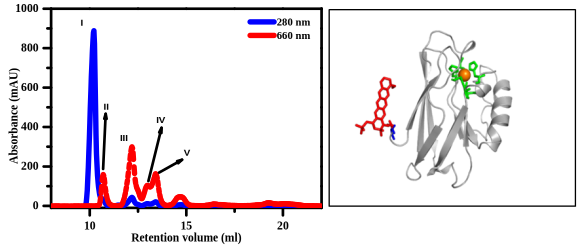
\includegraphics[width=0.8\textwidth]{peak_separation}
  \makeatletter
  \renewcommand{\fnum@figure}{\figurename~S\thefigure}
  \makeatother
  \caption{Peak separation: (a) Elution profile of Cu azurin sample after labeling and removal of free dye.
  \SI{280}{\nm} absorption that tells the presence of protein is shown in blue and \SI{660}{\nm} absrption that tells the presence of  dye is shown in red.
  The protein structure with the dye at Lys corresponding to peak-III is shown in the right. 
  {A proper structure will be replaced}}
  \label{SIfig: peak_sep}
\end{figure}
% \pagebreak
%==================BULK Switching=========================
\paragraph*{Fluorescence switching in bulk} Fluorescence measurements in bulk of different peaks of azurin-ATTO655 sample (Figure S\ref{SIfig: peak_sep}) were carried out to determine the FRET switching ratio.
The measurements were done in Cary Eclipse Spectrometer (Varian Inc. Agilent Technology, USA).
A \SI{50}{\nM} sample was excited with \SI{665}{\nm} and intensity was monitored above \SI{675}{\nm}.
Sodium ascorbate (reductant) and pottasium ferricyanide (oxidant) were added alternatively.
Among all the labeled position, peak-III showed maximum switching ratio and it's intensity change can be seen in Figure S\ref{SIfig: switching}.
Similarly Zn Azurin-ATTO655 showed little or no change in intensity.
\begin{figure}
  \centering
  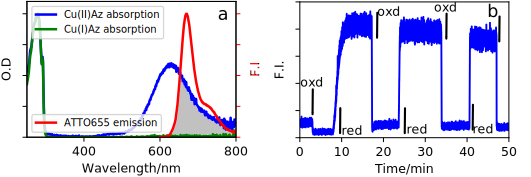
\includegraphics[width=\textwidth]{spectral_overlap_switching}
  \makeatletter
  \renewcommand{\fnum@figure}{\figurename~S\thefigure}
  \makeatother
  \caption{Spectral overlap and Bulk switching: (a) Absorption spectrum of Cu(II)azurin (blue), Cu(I)azurin (blue).
  The emission spectrum of ATTO655 (red) has a good overlap with the absorption of Cu(II)azurin to show high FRET. 
  (b) Fluorescence intensity of \SI{50}{\nM} CuAzurin-ATTO655 shows high intensity in the presence of reductant and low 
  intensity with oxidant.
  The switching ratio comes to be \SI{90}{\percent} satisfying the requirement for single-molecule FRET.}
  \label{SIfig: switching}
\end{figure}
%==================time trace Zn and Cu azurin=================
\begin{figure}
  \centering
  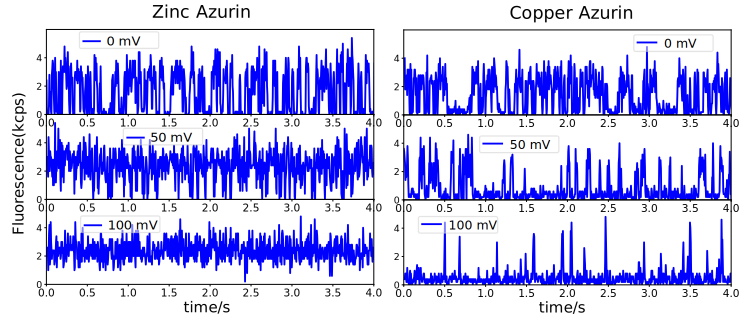
\includegraphics[width=\textwidth,keepaspectratio]{SI_timetrace_Zn_Cu}
  \makeatletter
  \renewcommand{\fnum@figure}{\figurename~S\thefigure}
  \makeatother
  \caption{Time traces of Zn Azurin (left) and of Cu Azurin(right) labeled with ATTO655 at different potential. 
  Above \SI{40}{\mV}, Cu-Azurin show swiching in the intensity due to changes in the oxidation state of the Copper metal center and below \SI{40}{\mV}, triplet blinking contributes to the switching as can be seen in the redox inactive Zn-Azurin.
  To keep the analysis simple, time traces above \SI{40}{\mV} were choosen for Cu azurin}
  \label{SIfig:tracecomparision}
\end{figure}
%===================lifetime and switching ration from time trace================
\begin{figure}
  \centering
  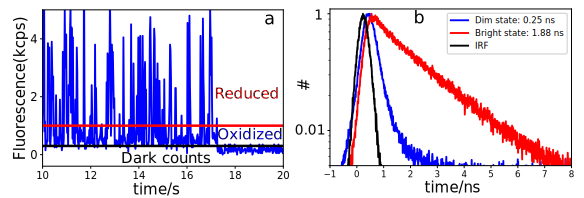
\includegraphics[width=\textwidth]{lifetime}
  \makeatletter
  \renewcommand{\fnum@figure}{\figurename~S\thefigure
}  \makeatother
  \caption{Single-molecule azurin switching and lifetime. (a) Time trace of a single Cu azurin at \SI{50}{\mV} with a binning time of \SI{50}{\ms}.
  Notice the three different labels indicated in the figure. Bright (Cu(I)) state as above the red line, oxidized state is between red and black and Dark counts are below the black line. The fact that the molecule doesn't go to the dark count label before being bleached shows that the transitions are due to Copper oxidation switching rather than triplet blinking of the dye.
  Once the fluorophore is bleached, no transitions were observavable.
  (b) The lifetime histogram corresponding to bright state (red), oxidized state (blue) and instrument response function (black).
  The lifetime of oxidized state is much shorter than the reduced state due to FRET quenching.}
  \label{SIfig: lifetime}
\end{figure}
%=====================FCS comparision=========================
\begin{figure}
  \centering
  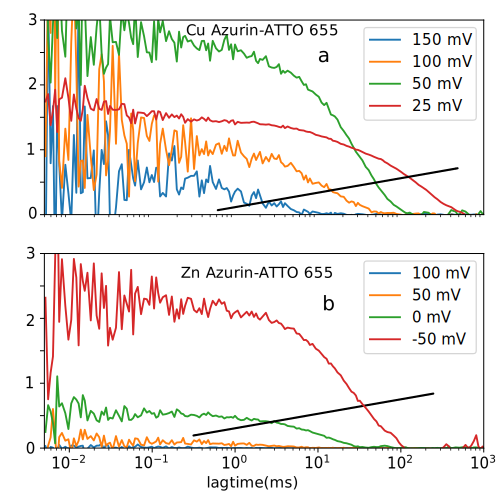
\includegraphics[width=\textwidth]{fcs_comparision}
  \makeatletter
  \renewcommand{\fnum@figure}{\figurename~S\thefigure}
  \makeatother
  \caption{Autocorrelation of time traces of Cuazurin-ATTO655 (a) and Znazurin-ATTO655 at different potential. 
  At lower potential, Cuazurin-ATTO655 has longer correlation time (on time) which shows that the molecule spends more time on the Cu(I) state.
  But below \SI{50}{\mV} the dye (ATTO655) starts to show triplet blinking.
  As potential is lowered the triplet blinking dominates.
  The Cu azurin study is focussed in the safe window of potential more than \SI{40}{\mV} where triplet blinking is absent.}
  \label{SIfig:fcscomparision}
\end{figure}
%===============================Slope: Nernst equation==================================
\begin{figure}
  \centering
  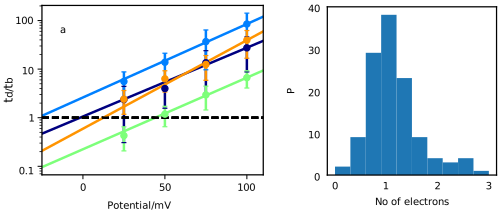
\includegraphics[width=\textwidth,keepaspectratio]{SI_potential_slope}
  \makeatletter
  \renewcommand{\fnum@figure}{\figurename~S\thefigure}
  \makeatother
  \caption{Fitting with Nernst equation with slope as variable parameters for  (a) Cu-Azurin ATTO655. 
  (b) The corresponding histogram of slopes obtained from the fitting shown in the left.T
  he distribution of slope is centered around \SI{59}{\mV} indicating that Cuazurin switching  involves only one electron.}
  \label{SIfig:potential_slope}
\end{figure}
%===================================Rate fit at all potential=============================
\begin{figure}
  \centering
  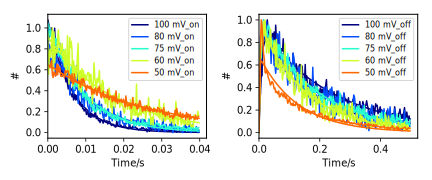
\includegraphics[width=\textwidth]{rate_fit_all_potential}
  \makeatletter
  \renewcommand{\fnum@figure}{\figurename~S\thefigure}
  \makeatother
  \caption{(a) Fitting of $on$ time distribution with monoexponential at different potential.
  (a) Fitting of $off$ time distribution with bi-exponential equation with rise time as shown in the main text at different potential.
  The output rate constants were plotted against potential (see main text)}
  \label{SIfig: rate_fit_all_potential}
\end{figure}
%===================================No of averaging points=================================
\begin{figure}
  \centering
  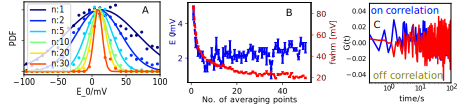
\includegraphics[width=\textwidth]{N_avgpoints_vs_fwhmwidth}
  \makeatletter
  \renewcommand{\fnum@figure}{\figurename~S\thefigure}
  \makeatother
  \caption{\textbf{No correlation dynamics.} Variation of midpoint potential and fwhm with the number of on and off times taken for averaging for the long trace shown in the main text (Figure-\ref{fig:long_azurin_trace}). At around $20~$ events, both $E_0$ and fwhm reaches palteu.
  The averaging of on-time and off-times for correlation and midpoint distribution were done every $20$ events.}
  \label{fig: N_avgpoints_vs_fwhmwidth}
\end{figure}
\paragraph*{}
\begin{figure}
  \centering
  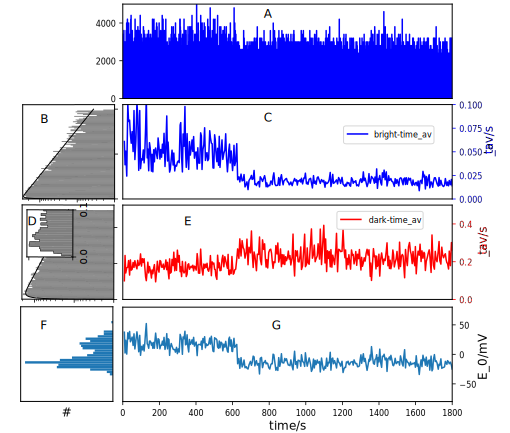
\includegraphics[width=\textwidth]{dynamic_trace_steps}
  \caption{\textbf{Two conformational state dynamics}}
  \label{SIfig:dynamic_trace_steps}
\end{figure}
%============on-off 2D histogram=============
\begin{figure}
  \centering
  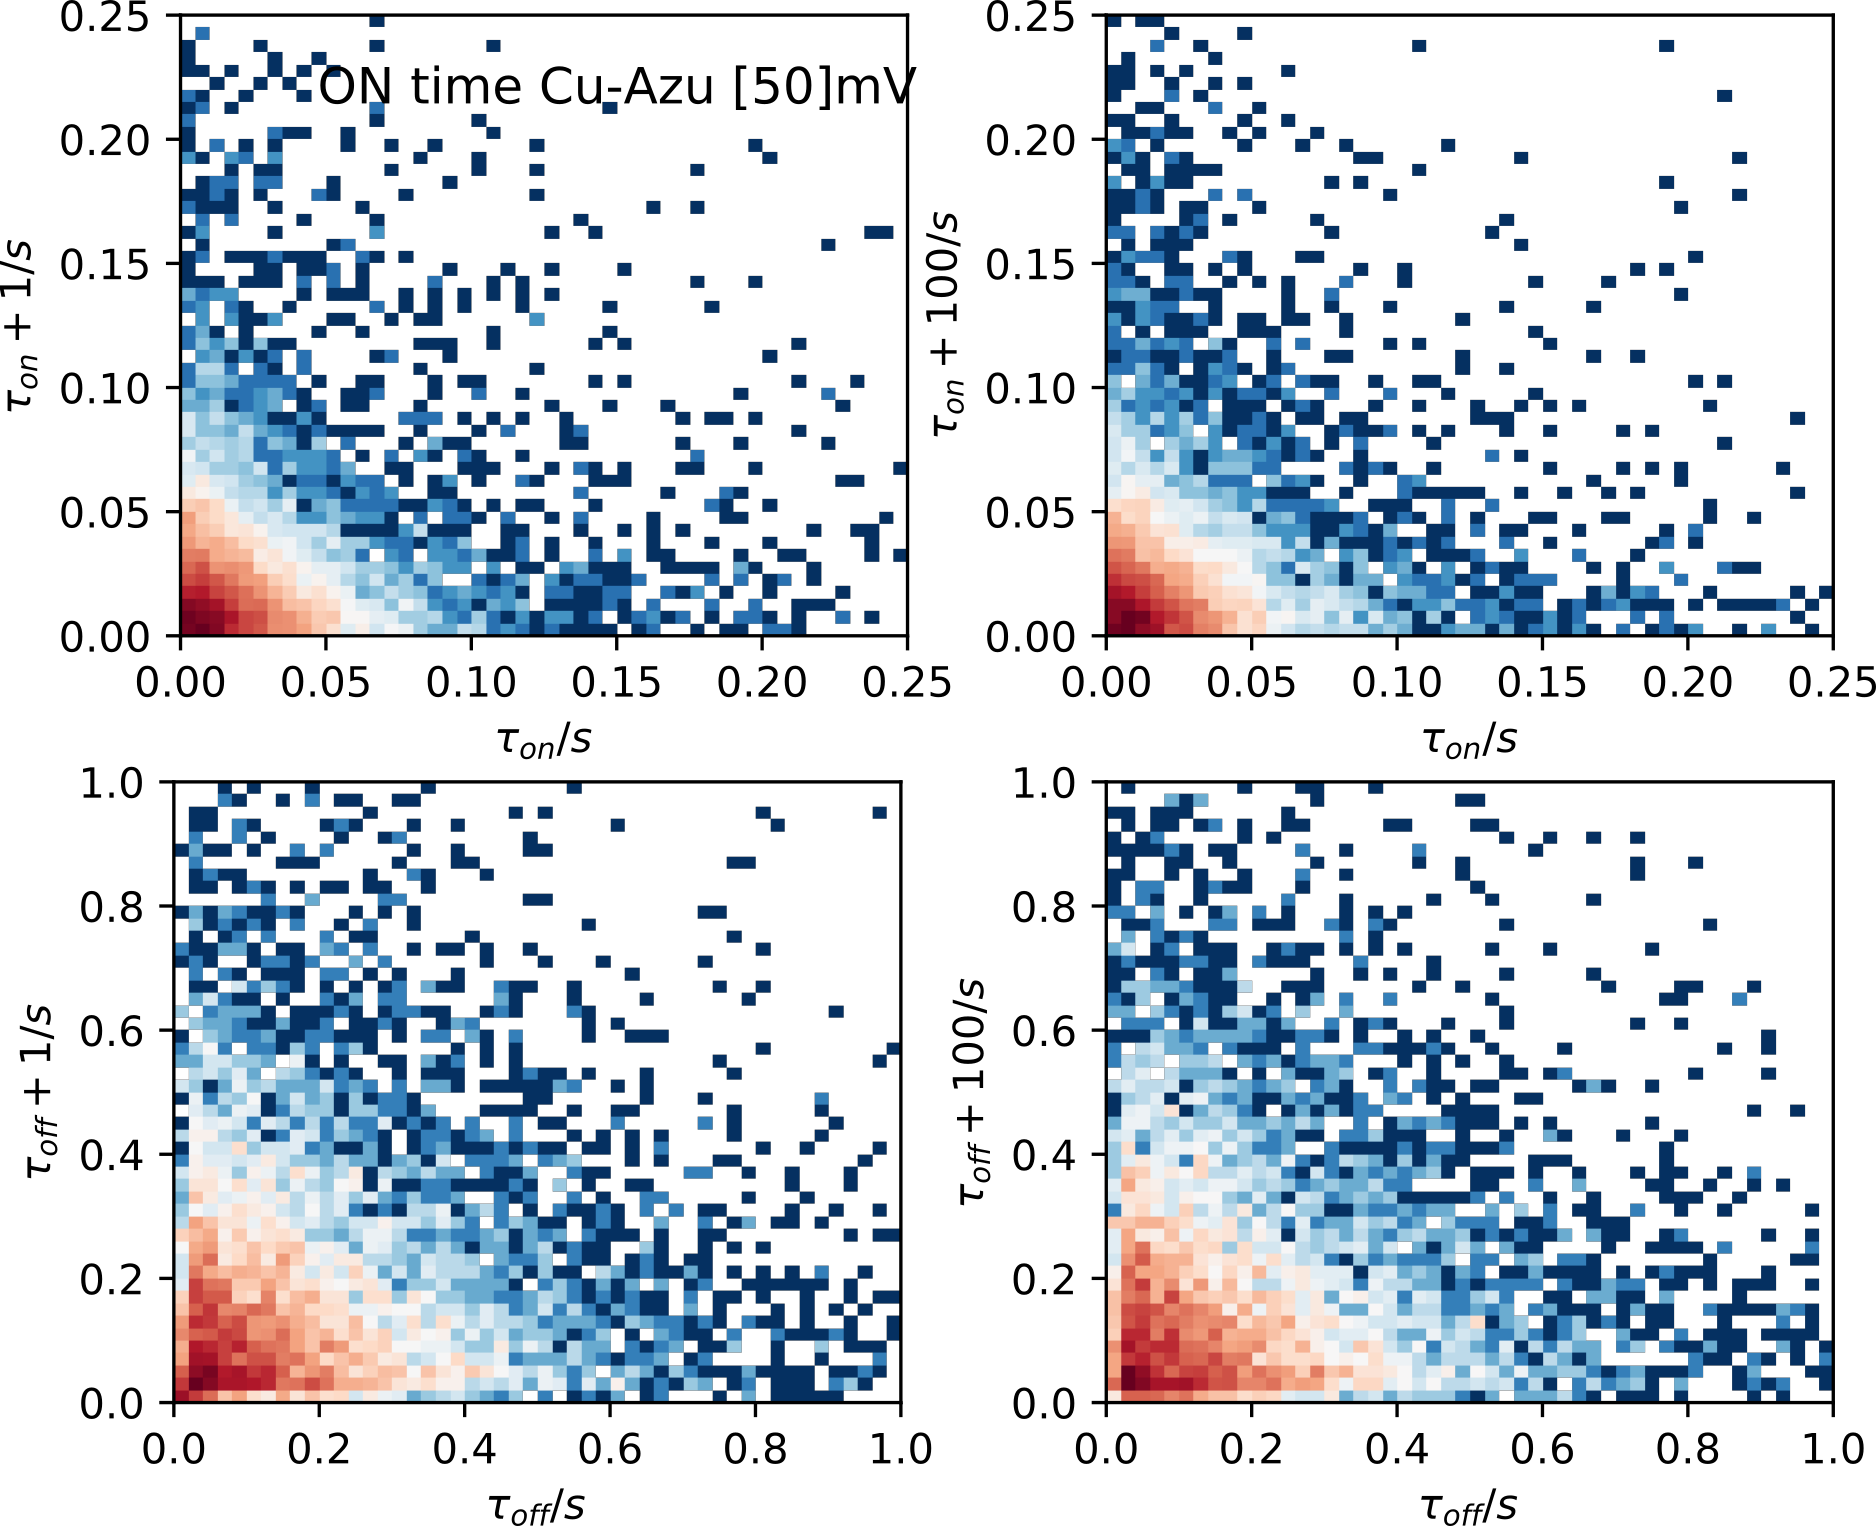
\includegraphics[width=\textwidth]{Figure_4_on_off_2D_100mV}
  \caption{\textbf{2D histogram: Cu-Azurin.}Two-dimensional correlation plot of a single azurin at \SI{50}{\mV} of(a) adjacent waiting time for oxidation ($t_{n}~and~t_{n+1}$) (b) two waiting times at a large separation of 100 ($t_{n}~and~t_{n+100}$) (c) The difference two dimensional histogram of (a) and (b).}
  \label{SIfig:onoff2D}
\end{figure}

\begin{figure}
  \centering
  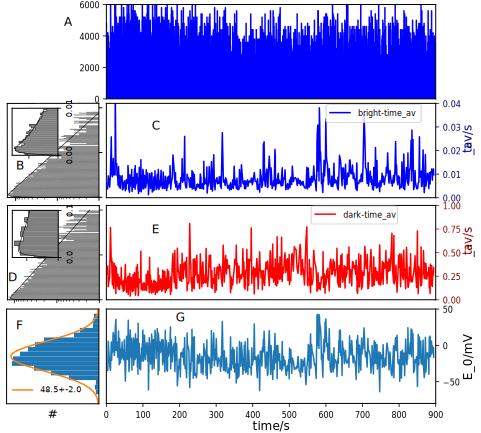
\includegraphics[width=\textwidth]{dynamic_Point_20_75mV_S105}
  \caption{\textbf{dynamic Point 20 75mV S105}}
  \label{SIfig:dynamic_Point_20_75mV_S105}
\end{figure}
\begin{figure}
  \centering
  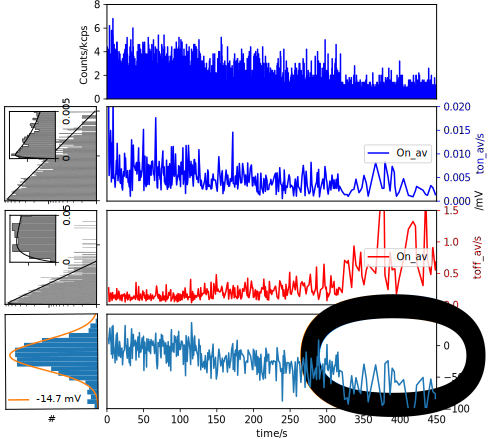
\includegraphics[width=\textwidth]{dynamic_Point_21_75mV_S105}
  \caption{\textbf{dynamic Point 20 75mV S105}}
  \label{SIfig:dynamic_Point_21_75mV_S105}
\end{figure}
\begin{figure}
  \centering
  \includegraphics[width=\textwidth]{Dynamic_corr_many}
  \caption{\textbf{More examples of Dynamic correlation.} 
  }
  \label{SIfig:Dynamic_corr_many}
\end{figure}
% \references{chapters/c4_azurin_sm/azurin}